%%%%%%%%%%%%%%%%%%%%%%%%%%%%%%%%%%%%%%%%%%%%%%%%%%%%%%%%%%%%%%%%%%%%%%%%%%%%%%%%%%%%
% Template for STAT 548 Qualifying Paper Report
% Author: Ben Bloem-Reddy <benbr@stat.ubc.ca>
% Date: Aug. 21, 2019
%%%%%%%%%%%%%%%%%%%%%%%%%%%%%%%%%%%%%%%%%%%%%%%%%%%%%%%%%%%%%%%%%%%%%%%%%%%%%%%%%%%%

% Note: You will get an empty bibliography warning when compiling until you include a citation.

\documentclass[10pt]{article}
% header.tex
% this is where you load pacakges, specify custom formats, etc.

\usepackage[left=1in,right=1in,top=1in,footskip=25pt]{geometry} 
% \usepackage{changepage}
\usepackage{amsmath,amsthm,amssymb,amsfonts}
\usepackage{mathtools}
% enumitem for custom lists
\usepackage{enumitem}
% Load dsfont this to get proper indicator function (bold 1) with \mathds{1}:
\usepackage{dsfont}
\usepackage{centernot}

\usepackage{bm}

\usepackage[usenames,dvipsnames]{xcolor}

\usepackage{tikz}
\usetikzlibrary{arrows.meta}

% set up commenting code (I will use this during marking)
\definecolor{CommentColor}{rgb}{0,.50,.50}
\newcounter{margincounter}
\newcommand{\displaycounter}{{\arabic{margincounter}}}
\newcommand{\incdisplaycounter}{{\stepcounter{margincounter}\arabic{margincounter}}}
\newcommand{\COMMENT}[1]{\textcolor{CommentColor}{$\,^{(\incdisplaycounter)}$}\marginpar{\scriptsize\textcolor{CommentColor}{ {\tiny $(\displaycounter)$} #1}}}

% \DeclareMathOperator{\deg}{deg}

\usepackage{appendix}

% set up graphics
\usepackage{graphicx}
\DeclareGraphicsExtensions{.pdf,.png,.jpg}
\graphicspath{ {fig/} }

\usepackage[sorting=nyt,backend=biber,bibstyle=alphabetic,citestyle=alphabetic,giveninits=true]{biblatex}

\usepackage{fancyhdr}
\pagestyle{fancy}
\setlength{\headheight}{40pt}

%%%%%%%%%%%%%%%%%%%%%%%%%%%%%%%%%%%%%%%%%%%%%%%%%%%%%%%%%%%%%%%%%%%%%%%%%%%%%%%%%%%%
% most other packages you might use should be loaded before hyperref
%%%%%%%%%%%%%%%%%%%%%%%%%%%%%%%%%%%%%%%%%%%%%%%%%%%%%%%%%%%%%%%%%%%%%%%%%%%%%%%%%%%%

% Set up hyperlinks:
\definecolor{RefColor}{rgb}{0,0,.65}
\usepackage[colorlinks,linkcolor=RefColor,citecolor=RefColor,urlcolor=RefColor]{hyperref}

\usepackage[capitalize]{cleveref}
\crefname{appsec}{Appendix}{Appendices} % you can tell cleveref what to call things
% defs.tex
% this is where you define custom notation, commands, etc.


%%
% full alphabets of different styles
%%

% bf series
\def\bfA{\mathbf{A}}
\def\bfB{\mathbf{B}}
\def\bfC{\mathbf{C}}
\def\bfD{\mathbf{D}}
\def\bfE{\mathbf{E}}
\def\bfF{\mathbf{F}}
\def\bfG{\mathbf{G}}
\def\bfH{\mathbf{H}}
\def\bfI{\mathbf{I}}
\def\bfJ{\mathbf{J}}
\def\bfK{\mathbf{K}}
\def\bfL{\mathbf{L}}
\def\bfM{\mathbf{M}}
\def\bfN{\mathbf{N}}
\def\bfO{\mathbf{O}}
\def\bfP{\mathbf{P}}
\def\bfQ{\mathbf{Q}}
\def\bfR{\mathbf{R}}
\def\bfS{\mathbf{S}}
\def\bfT{\mathbf{T}}
\def\bfU{\mathbf{U}}
\def\bfV{\mathbf{V}}
\def\bfW{\mathbf{W}}
\def\bfX{\mathbf{X}}
\def\bfY{\mathbf{Y}}
\def\bfZ{\mathbf{Z}}

% bb series
\def\bbA{\mathbb{A}}
\def\bbB{\mathbb{B}}
\def\bbC{\mathbb{C}}
\def\bbD{\mathbb{D}}
\def\bbE{\mathbb{E}}
\def\bbF{\mathbb{F}}
\def\bbG{\mathbb{G}}
\def\bbH{\mathbb{H}}
\def\bbI{\mathbb{I}}
\def\bbJ{\mathbb{J}}
\def\bbK{\mathbb{K}}
\def\bbL{\mathbb{L}}
\def\bbM{\mathbb{M}}
\def\bbN{\mathbb{N}}
\def\bbO{\mathbb{O}}
\def\bbP{\mathbb{P}}
\def\bbQ{\mathbb{Q}}
\def\bbR{\mathbb{R}}
\def\bbS{\mathbb{S}}
\def\bbT{\mathbb{T}}
\def\bbU{\mathbb{U}}
\def\bbV{\mathbb{V}}
\def\bbW{\mathbb{W}}
\def\bbX{\mathbb{X}}
\def\bbY{\mathbb{Y}}
\def\bbZ{\mathbb{Z}}

% cal series
\def\calA{\mathcal{A}}
\def\calB{\mathcal{B}}
\def\calC{\mathcal{C}}
\def\calD{\mathcal{D}}
\def\calE{\mathcal{E}}
\def\calF{\mathcal{F}}
\def\calG{\mathcal{G}}
\def\calH{\mathcal{H}}
\def\calI{\mathcal{I}}
\def\calJ{\mathcal{J}}
\def\calK{\mathcal{K}}
\def\calL{\mathcal{L}}
\def\calM{\mathcal{M}}
\def\calN{\mathcal{N}}
\def\calO{\mathcal{O}}
\def\calP{\mathcal{P}}
\def\calQ{\mathcal{Q}}
\def\calR{\mathcal{R}}
\def\calS{\mathcal{S}}
\def\calT{\mathcal{T}}
\def\calU{\mathcal{U}}
\def\calV{\mathcal{V}}
\def\calW{\mathcal{W}}
\def\calX{\mathcal{X}}
\def\calY{\mathcal{Y}}
\def\calZ{\mathcal{Z}}


%%%%%%%%%%%%%%%%%%%%%%%%%%%%%%%%%%%%%%%%%%%%%%%%%%%%%%%%%%
% text short-cuts
\def\iid{i.i.d.\ } %i.i.d.
\def\ie{i.e.\ }
\def\eg{e.g.\ }
\def\Polya{P\'{o}lya\ }
%%%%%%%%%%%%%%%%%%%%%%%%%%%%%%%%%%%%%%%%%%%%%%%%%%%%%%%%%%

%%%%%%%%%%%%%%%%%%%%%%%%%%%%%%%%%%%%%%%%%%%%%%%%%%%%%%%%%%
% quasi-universal probabilistic and mathematical notation
% my preferences (modulo publication conventions, and clashes like random vectors):
%   vectors: bold, lowercase
%   matrices: bold, uppercase
%   operators: blackboard (e.g., \mathbb{E}), uppercase
%   sets, spaces: calligraphic, uppercase
%   random variables: normal font, uppercase
%   deterministic quantities: normal font, lowercase
%%%%%%%%%%%%%%%%%%%%%%%%%%%%%%%%%%%%%%%%%%%%%%%%%%%%%%%%%%

% operators
\def\P{\bbP} %fundamental probability
\def\E{\bbE} %expectation
% conditional expectation
\DeclarePairedDelimiterX\bigCond[2]{[}{]}{#1 \;\delimsize\vert\; #2}
\newcommand{\conditional}[3][]{\bbE_{#1}\bigCond*{#2}{#3}}
\def\Law{\mathcal{L}} %law; this is by convention in the literature
\def\indicator{\mathds{1}} % indicator function

% sets and groups
\def\borel{\calB} %Borel sets
\def\sigAlg{\calA} %sigma-algebra
\def\filtration{\calF} %filtration
\def\grp{\calG} %group

% binary relations
\def\condind{{\perp\!\!\!\perp}} %independence/conditional independence
\def\equdist{\stackrel{\text{\rm\tiny d}}{=}} %equal in distribution
\def\equas{\stackrel{\text{\rm\tiny a.s.}}{=}} %euqal amost surely
\def\simiid{\sim_{\mbox{\tiny iid}}} %sampled i.i.d

% common vectors and matrices
\def\onevec{\mathbf{1}}
\def\iden{\mathbf{I}} % identity matrix
\def\supp{\text{\rm supp}}

% misc
% floor and ceiling
\DeclarePairedDelimiter{\ceilpair}{\lceil}{\rceil}
\DeclarePairedDelimiter{\floor}{\lfloor}{\rfloor}
\newcommand{\argdot}{{\,\vcenter{\hbox{\tiny$\bullet$}}\,}} %generic argument dot
%%%%%%%%%%%%%%%%%%%%%%%%%%%%%%%%%%%%%%%%%%%%%%%%%%%%%%%%%%

%%%%%%%%%%%%%%%%%%%%%%%%%%%%%%%%%%%%%%%%%%%%%%%%%%%%%%%%%%
%% some distributions
% continuous
\def\UnifDist{\text{\rm Unif}}
\def\BetaDist{\text{\rm Beta}}
\def\ExpDist{\text{\rm Exp}}
\def\GammaDist{\text{\rm Gamma}}
% \def\GenGammaDist{\text{\rm GGa}} %Generalized Gamma

% discrete
\def\BernDist{\text{\rm Bernoulli}}
\def\BinomDist{\text{\rm Binomial}}
\def\PoissonPlus{\text{\rm Poisson}_{+}}
\def\PoissonDist{\text{\rm Poisson}}
\def\NBPlus{\text{\rm NB}_{+}}
\def\NBDist{\text{\rm NB}}
\def\GeomDist{\text{\rm Geom}}
% \def\CRP{\text{\rm CRP}}
% \def\EGP{\text{\rm EGP}}
% \def\MittagLeffler{\text{\rm ML}}
%%%%%%%%%%%%%%%%%%%%%%%%%%%%%%%%%%%%%%%%%%%%%%%%%%%%%%%%%%

%%%%%%%%%%%%%%%%%%%%%%%%%%%%%%%%%%%%%%%%%%%%%%%%%%%%%%%%%%
% Project-specific notation should go here
% (Because it's at the end of the file, it can overwrite anything that came before.)

%e.g.,
\def\Laplacian{\calL}
\def\P{\calP}

% combinatorial objects
\def\perm{\sigma} %fixed permutation
\def\Perm{\Sigma} %random permutation
\def\part{\pi} %fixed partition
\def\Part{\Pi} %random partition


%%%%%%%%%%%%%%%%%%%%%%%%%%%%%%%%%%%%%%%%%%%%%%%%%%%%%%%%%%

%%%%%%%%%%%%%%%%%%%%%%%%%%%%%%%%%%%%%%%%%%%%%%%%%%%%%%%%%%%%%%%%%%%%%%%%%%%%%%%%%

% your title/author/date information go here
\title{\LaTeX\ Template for STAT 548 Qualifying Paper Report} % replace with your title
\author{Benjamin Bloem-Reddy} % replace with your name
\date{\today} % replace with your submission date

\bibliography{../../ref/qp-bib.bib} % add the title of your bibliography file

% start of document
\begin{document}

\maketitle

\section{preliminary notes}

\subsection{abstract and introduction}

\begin{itemize}
    \item use gaussian processes to learn unknown functions ``in a manner that permits one to utilize prior information about their properties''
    \item the idea appears to be that we want a gp for when the input space is an undirected graph
    \item and the ``spde'' characterization of matern gps leads to a gp on undirected graphs that is easy to work with
    \item i think gps are characterized by their mean and (more importantly) covariance functions\footnote{I think covariance function and kernel are the same thing?}
    \item ``predicting street congestion with a road network''; this is sort of like predicting a cost or constraint, isn't it?
    \item ``we study GPs whose inputs or outputs are indexed by the vertices of an undirected graph, where each edge between adjacent nodes is assigned a positive weight''
    \item gaussian markov random fields (gmrf) are relevant here
    \item it seems that, for graphs with finitely many nodes, the covariance functions can be viewed as ``parameterized structured covariance matrices that encode dependence between vertices.''
    \item can we work with infinite graphs, or just finite ones?
    \item so there have been explorations of kernels for graph gps before, but apparently this attempt to port over a type of matern (which is commonly used for $\mathbb R^n$) for graphs is new?
    \item in ``normal'' contexts, you can define a matern kernel via spde representation; that appears to be the approach taken for graph gps here
    \item as an alternative to the spde derivation/version, there is also a fourier feature approach
    \item graph gp matern kernels converge to euclidean gp matern kernels when the graph becomes more dense?
\end{itemize}

\subsection{gaussian processes}

\begin{itemize}
    \item do i need to worry about the sigma field on the space of functions? I am guessing not for the purposes of this project
    \item explanation of gp is a bit confusing. $\bm x \in X^n$ is one point $(x_1, \dots, x_n)$, right? and then $f(\bm x) = f(x_1, \dots, x_n)$ is a real number, right? do they mean $\left( f(x_1), \dots, f(x_n) \right)$?
    \item maybe put anothe rway, i don't understand how the given description jives with the regular notion that a gp is a sequence of rando mvariables such that all finite collections are multivariate-normal distributed
    \item anyway, we can assume the mean function $\bm mu$ is zero, so forget about that; we focus on the kernel $\bm{K_{xx}}$
    \item so the intuitive idea seems to be that we start with some gp (our ``prior'' gp?), and then given our data, we get a new, updated, ``posterior'' gp, given the data?
    \item i guess it's worth noting that both (1) and (2) involve matrix inversion, which I think is computationall expensive
    \item ``mean-square differentiability'' seems to be some kind of stochastic process notion of a derivative, which is probably not relevant for this project
    \item from \href{https://en.wikipedia.org/wiki/Mat%C3%A9rn_covariance_function}{Wikipedia}, it seems that matern kernels are functions of the distance between pairs of points.
    \item matern gps can be put on the sphere and torus
    \item 
\end{itemize}

\subsubsection{gps on graphs}

\begin{itemize}
    \item i guess if a a matern kernel for a regular gp is a function of the distance between two points, then to create a matern kernel for a graph gp, we need some kind of notion of distance on the graph.
    \item i guess if we take a step back, then if a gaussian process ``is'' in some sense a distribution on a space of function, then we can ask: functions from what to what? If $\mathbb R^n$ to $\mathbb R^n$ is standard, then here we are exploring i guess the possibility that one or both of domain and codomain are weighted graphs?
\end{itemize}

\subsection{matern gps on graphs}

\begin{itemize}
    \item so to define a matern gp on a graph, we need to convert (6) and (7) to some kind of ``graph spde?''
    \item ``Note that since a graph is a finite set, such a Gaussian process can be viewed as a multivariate Gaussian whose indices are the graph's nodes''
    \item so no gps on infinite graphs?
    \item (8): definition of graph laplacian; so for a finite graph it's just a certain matrix (\href{https://mbernste.github.io/posts/laplacian_matrix/}{link})
    \item don't really get what's going on with the matrix $\Phi(\bm{\Delta})$. taylor expansions don't always exist, right? and what does it mean to plug a matrix into the taylor expansion of a function from $\mathbb R$ to $\mathbb R$?
    \item the mathematical derivations seem to have some serious gaps, at least for my level
    \item 
\end{itemize}

\section{links that might be relevant}

\begin{itemize}
    \item \href{https://math.stackexchange.com/questions/6258/matrices-commute-if-and-only-if-they-share-a-common-basis-of-eigenvectors}{commuting matrices}; just thought it seemed interesting; maybe not relevant for this project
    \item \href{https://en.wikipedia.org/wiki/Eigendecomposition_of_a_matrix#Real_symmetric_matrices}{eigendecomp}; thinking whether the positive-definiteness of the matrix $\bm{\Delta}$ is relevant?
    \item \href{https://en.wikipedia.org/wiki/Definite_matrix}{definite matrices}; same as above
    \item \href{https://math.stackexchange.com/questions/82467/eigenvectors-of-real-symmetric-matrices-are-orthogonal}{orthogonal eigenvectors}; related to above
    \item \href{https://en.wikipedia.org/wiki/Taylor_series#:~:text=The%20partial%20sum%20formed%20by,more%20accurate%20as%20n%20increases.}{taylor series}; what conditions do we need for $\Phi$ to have a taylor expansion?
    \item \href{https://en.wikipedia.org/wiki/Matrix_exponential}{matrix exponential}; because the matrix exponential appears to be used
\end{itemize}

% summary section
% !TEX root = ../main.tex

% Summary section

\section{Publication-style review}

\subsection{Summary}

The paper \cite{pmlr-v130-borovitskiy21a} introduces a new type of kernel for a Gaussian process on a weighted graph. In particular, the popular Mat\'{e}rn kernel for Gaussian processes on Euclidean space is in some sense converted to a graph-theoretic kernel by replacing the Euclidean Laplace operator with the graph-theoretic Laplacian matrix. Mathematical details of the derivation are not provided in significant detail. As computational efficiency when working with large datasets is a general concern when using Gaussian processes, the authors also discuss computational aspects of the graph Mat\'{e}rn Gaussian process. Sparse graphs generally lead to faster computation, and various approximation techniques are also discussed, both for regression and classification. The authors also provide two comparisons of graph Mat\'{e}rn kernel with other kernels, and the performance is roughly comparable. It is not clear when one kernel might be preferable to another.

\subsection{High-level comments on strengths and weaknesses}

The main strength of the paper is the introduction of a new (Mat\'{e}rn) kernel for Gaussian processes on graphs. Furthermore, it is at least of theoretical interest that the new kernel is so closely related to the popular Mat\'{e}rn kernel for Gaussian processes on Euclidean space. The main weaknesses of the paper are twofold. First, the graph Mat\'{e}rn kernel does not appear to meaningfully outperform pre-existing alternatives, although this is not a significant weakness. Second, and perhaps slightly more signifcant, the the mathematical detail in \cite{pmlr-v130-borovitskiy21a} is relatively scarce and it is not obvious that the target audience will be able to reconstruct the mathematical derivations. In relation to other work, \cite{pmlr-v130-borovitskiy21a} is quite similar at least in inspiration to the authors' previous work \cite{NEURIPS2020_92bf5e62}, which applies a very similar trick in the replacement of the Euclidean Laplace operator with a related Laplace operator---the Laplace-Beltrami operator in the case of \cite{NEURIPS2020_92bf5e62}, and the graph Laplacian in the case of \cite{pmlr-v130-borovitskiy21a}.

\subsection{Originality}

It is not completely obvious precisely what is novel in the paper in question, because there doesn't appear to be any phrase along the lines of ``We present a novel\dots'' or ``We introduce\dots'' that would make clear exactly what novel work has been done by the authors. It \textit{appears} that, while Gaussian processes on Euclidean space are well known and Gaussian processes on graphs have been studied, the paper in question is the first to essentially port the Mat\'{e}rn kernel version of a Gaussian process from Eucliean space to the graph context. The work is a combination of prior techniques in the sense that both Gaussian processes on graphs, and Mat\'{e}rn kernels on Euclidean space, have both been studied (separately, apparently). If the work in question is the first to introduce Mat\'{e}rn Gaussian processes on graphs, then it obviously differentiates itself from prior work. Regarding the question of adequate citations, I think it depends to a significant extent on the novelty of the work. If the paper \textit{is} the first to introduce Mat\'{e}rn Gaussian processes on graphs, then by dint of its originality there will not be as as much prior work to cite. If it is not, then the appears to suffer from inadequate citations reflecting this fact, particularly in Sections 2.2 and 3.

\subsection{Quality}

It is important to keep one's audience in mind when presenting new work. The lead author is a pure mathematician by training and is presenting his work to an audience presumably consisting of statisticians, so there is presumably a large gap in mathematical knowledge beween the author and his audience. It seems very unlikely that many statisticians will have any particular familiarity with, for example, stochastic partial differential equations, heat semigroups, or Riemannian manifolds. Given this gap in mathematical knowledge it appears that the paper in question may be short in detail for some of its mathematical derivations, for example precisely how the standard Mat\'{e}rn kernel for $\mathbb R^n$ is converted to to a graph-theoretic version. If statisticians are happy to ignore technical details then the paper might be considered technically sound, especially if we presume that the lead author's mathematical training reduces the chance of his results being erroneous. On the other hand, if the audience is interested in understanding precisely how the graph-theoretic Mat\'{e}rn kernel was derived, then the paper appears short on mathematical justifications. Indeed, the word ``proof'' does not seem to appear in the paper. The authors appear to honestly present the strengths and weaknesses of their work insofar as they do not claim that Mat\'{e}rn Gaussian processes necessarily represent a major advance, especially since their own empirical results do not appear to show significantly improved performance compared to other kernels.

\subsection{Clarity}

The writing and presentation generally seem clear, modulo the aforementioned potential issues with a lack of mathematical clarity. The question of whether the paper ``adequately informs the reader'' of course depends on the reader's level of mathematical sophistication---see the above discussion on this point. Regarding code, the authors have provided code in a GitHub repository.

\subsection{Significance}

The results appear to be important insofar as they present a new kernel for Gaussian processes on graphs, and in particular it is interesting that a common kernel for Euclidean space has been ``ported'' over to graphs. The mathematical techniques used appear closely related (at least in spirit) to the techniques employed in the authors' previous paper \cite{NEURIPS2020_92bf5e62}

It is unclear whether the mathematical techniques employed in the paper are ripe for further exploitation, at least in part because I don't fully understand then, nor are they thoroughly described. The authors' own experiments do not suggest that graph Mat\'{e}rn Gaussian processes blow away the competition, but with only two comparisons provided, it is too early to judge. At any rate, requiring that a new technique supercede all existing techniques is too high a bar. It is not clear that the authors provide ``unique data'' or ``unique conclusions about existing data'', and as described above, it is hard to evaluate their theoretical approach.

\subsection{List of questions for the authors}

\begin{enumerate}
    \item Where and how can I learn more about the derivations and convergence results in this paper?
    \item Do you have any expectations regarding when the Mat\'{e}rn graph Gaussian process might perform better or worse than alternative kernels, both in terms of accuracy and computational efficiency? (Might the answer to this question depend both on the characteristics of the graph, the dataset itself and the desired type of prediction?)
    \item What if anything is impeding the application of Mat\'{e}rn kernels for Gaussian processes on directed and/or infinite graphs?
\end{enumerate}

\newpage
\subsection{Technical/methodological summary}

\subsubsection{Related literature and broader context}

% brief discussion of gaussian processes here
% then history of GPs on graphs
% maybe then discussion of different kernels for GPs on graphs
% (include citations)

A stochastic process $X$ on parameter space $T$ is said to be \textit{Gaussian} if the random variable $\sum_{i = 1}^n c_i X_{t_i}$ is Gaussian, for any choice of $n \in \mathbb N$, $t_1, \dots, t_n \in T$, and $c_1, \dots, c_n \in \mathbb R$ \cite{kallenberg}. Gaussian processes have been studied theoretically for at least a century, since the archetypal stochastic process, Brownian motion, is itself Gaussian \cite{kallenberg}. However, it appears that only in the last few decades have Gaussian processes become a significant tool in statistics and machine learning \cite{rw}.

By Lemma 14.1 of \cite{kallenberg}, the distribution of a Gaussian process $X$ is uniquely determined by the functions

\begin{equation}\label{eq:gaus_1}
    m_t = \mathrm E X_t, \quad r_{s, t} = \text{Cov}(X_s, X_t)
\end{equation}

for $s, t \in T$. However, among applied practitioners it appears that when using Gaussian processes, much more attention is paid to the covariance function than the mean function \cite{garnett_bayesoptbook_2023}. \textcolor{red}{(The precise details regarding the relationship between the regular covariance operation as in (\ref{eq:gaus_1}), and covariance functions more generally, will not be explored in this report.)}

The standard definition of a stochastic process is a sequence of random variables $X = \left\{ X_t \colon t \in T \right\}$ over a parameter space $T$, which only requires the existence of some original probability space $\left( \Omega, \mathcal F, \mathbb P \right)$ and a (measurable) state space $(S, \mathcal S)$. This abstract definition permits the possibility that a stochastic process may be defined not only on Euclidean space, but also on other spaces, such as graphs \cite{grimmett}. Gaussian processes in particular are typically employed with Euclidean space as domain and codomain, but there is nothing in principle preventing Gaussian processes being defined on the vertices of a graph $G = (V, E)$, i.e. allowing $\Omega = V$. Indeed, this has been explored, as for example in \cite{kondor2002diffusion}. One of the key challenges in using Gaussian processes on graphs has been finding proper covariance functions, as explained in \cite{kondor2002diffusion}, since covariance functions (or ``kernels'') are required to be symmetric and positive semi-definite.

In the work \cite{pmlr-v130-borovitskiy21a}, a new kernel for Gaussian processes on graphs is explored, in some sense deriving a graph-theoretic version of the popular Mat\'{e}rn kernel for Gaussian processes on Euclidean space. The Euclidean Mat\'{e}rn kernel is a function $C_{\nu} \colon \mathbb R^d \to \mathbb R$ given by

\begin{equation}\label{eq:mat_1}
    C_{\nu}(d) = \frac{2^{1 - \nu}}{\Gamma(\nu)} \left(\sqrt{2 \nu} \frac{d}{\ell}\right)^{\nu} K_{\nu}\left(\sqrt{2 \nu} \frac{d}{\ell},\right),
\end{equation}

where $d$ is the Euclidean distance between points $\bm x, \bm x' \in \mathbb R^n$; $\nu, \ell > 0$; $\Gamma$ refers to the gamma function and $K_{\nu}$ is the modified Bessel function of the second kind \cite{rw}. In \ref{sec:method}, we will explore the derivation of the Mat\'{e}rn kernel for Gaussian processes on graphs.

\textcolor{red}{(The paper \cite{pmlr-v130-borovitskiy21a} also discusses a graph-theoretic version of the squared exponential kernel, which is related to the Mat\'{e}rn kernel. However, due to space limitations, this report will focus on the Mat\'{e}rn kernel.)}

\subsubsection{Proposed methodology and theoretical properties}\label{sec:method}

There does not appears to be a ``proposed methodology'' in \cite{pmlr-v130-borovitskiy21a}, insofar as the main contribution is a new kernel for Gaussian processes on graphs---presumably any existing method of using Gaussian processes on graphs can be used with the new kernel. Therefore, this section will focus on explaining whatever theoretical aspects of \cite{pmlr-v130-borovitskiy21a} that can reasonably be explained, given space limitations.

The paper \cite{pmlr-v130-borovitskiy21a} refers to the paper \cite{whittle1963stochastic} in support of a claim that a Gaussian process $f$ on $\mathbb R^d$ with Mat\'{e}rn kernel as in (\ref{eq:mat_1}) satisfies the stochastic partial differential equation

\begin{equation}\label{eq:spde_mat}
    \left(\frac{2\nu}{\kappa^2} - \Delta\right)^{\frac{\nu}{2} + \frac{d}{4}}f = \mathcal W,
\end{equation}

where $\nu$ and $\kappa$ are parameters, $\Delta$ is the Laplace operator and $\mathcal W$ is Gaussian white noise. Unfortunately, the paper \cite{whittle1963stochastic} cannot be located in either the Simon Fraser University Library, or the University of British Columbia library, so this claim cannot investigated in further detail.

In order to derive a graph-theoretic version of the Mat\'{e}rn kernel, the authors of \cite{pmlr-v130-borovitskiy21a} focus on the characterization of a Gaussian process as in (\ref{eq:spde_mat}). Although the derivation is not totally clear, a key step in the derivation appears to be replacing the Euclidean Laplace operator $\Delta$ with the Laplacian matrix $\bm \Delta$, which is a graph-theoretic analogue of the Euclidean Laplace operator $\Delta$. (Indeed, this appears to be a very similar at least in spirit to the maneuver used by the authors in their previous work \cite{NEURIPS2020_92bf5e62}, in which they replace the Euclidean Laplace operator in (\ref{eq:spde_mat}) with its Riemannian generalization, the Laplace-Beltrami operator. This substitution leads to the development of a Mat\'{e}rn Gaussian process on Riemannian manifolds in \cite{NEURIPS2020_92bf5e62}.)

The derivation can be at least partly explained as follows. First assume that the function $\Phi \colon \mathbb R \to \mathbb R$ as defined in \cite{pmlr-v130-borovitskiy21a} is analytic, roughly meaning that it is equal to its Taylor series, so we can write

\begin{equation}\label{eq:phi_1}
    \Phi(z) = a_0 + a_1 z + a_2 z^2 + \dots \, .
\end{equation}

If we then consider a diagonal matrix

\[
    \mathbf D = 
    \begin{pmatrix}
        d_1 & 0 & 0 & \ldots & 0 \\
        0 & d_2 & 0 & \ldots & 0 \\
        0 & 0 & d_3 & \ldots & 0 \\
        \vdots & \vdots & \vdots & \ddots & \vdots \\
        0 & 0 & 0 & \ldots & d_n
    \end{pmatrix},
\]

and we plug this into $\Phi$, then we can write

\begin{align*} % \label{eq:phi_1}
    \Phi(\mathbf D) &= a_0 + a_1 \mathbf D + a_2 \mathbf D^2 + \dots\\
    \\
    &= a_0 \mathbf I + a_1 
    \begin{pmatrix}
        d_1 & 0 & 0 & \ldots & 0 \\
        0 & d_2 & 0 & \ldots & 0 \\
        0 & 0 & d_3 & \ldots & 0 \\
        \vdots & \vdots & \vdots & \ddots & \vdots \\
        0 & 0 & 0 & \ldots & d_n
    \end{pmatrix}
    + a_2
    \begin{pmatrix}
        d_1^2 & 0 & 0 & \ldots & 0 \\
        0 & d_2^2 & 0 & \ldots & 0 \\
        0 & 0 & d_3^2 & \ldots & 0 \\
        \vdots & \vdots & \vdots & \ddots & \vdots \\
        0 & 0 & 0 & \ldots & d_n^2
    \end{pmatrix}
    + \dots \\
    \\
    &= 
    \begin{pmatrix}
        \Phi(d_1) & 0 & 0 & \ldots & 0 \\
        0 & \Phi(d_2) & 0 & \ldots & 0 \\
        0 & 0 & \Phi(d_3) & \ldots & 0 \\
        \vdots & \vdots & \vdots & \ddots & \vdots \\
        0 & 0 & 0 & \ldots & \Phi(d_n)
    \end{pmatrix}.
\end{align*}

Now, if $\mathbf O$ is an orthogonal matrix, then note that

\begin{align*}
    (\mathbf{ODO}^\intercal)^n &= \underbrace{(\mathbf{ODO}^\intercal)\dots(\mathbf{ODO}^\intercal)}_{n \text{ times}}\\
    &= \mathbf{O}\mathbf D^n \mathbf{O}^\intercal,
\end{align*}

so we conclude that

\begin{align*}
    \Phi(\mathbf \Delta) &= \Phi(\mathbf{U \Lambda U}^\intercal) \\
    &= a_0 + a_1 \mathbf{U \Lambda U}^\intercal + a_2 (\mathbf{U \Lambda U}^\intercal)^2 + \dots\\
    &= \mathbf U \Phi(\mathbf \Lambda) \mathbf{U}^\intercal,
\end{align*}

which is consistent with (9) in \cite{pmlr-v130-borovitskiy21a}.

The remainder of the argument, namely proceeding from (10) to (11) in \cite{pmlr-v130-borovitskiy21a}, is not totally clear, since it's not obvious where the matrices $\mathbf U$ and $\mathbf U^\intercal$ have gone. However, it seems possible that their disappearance is related to the invariance of $\bm{\mathcal W} \sim \mathrm N(\mathbf 0, \mathbf I)$ under orthogonal transformations.

\subsubsection{Computational complexity, crucial aspects and potential bottlenecks}

Gaussian processes, in and of themselves, are simply stochastic processes as described earlier, so it may only make sense to discuss computational performance in the context of a specific manner of use of Gaussian processes. As such, since \cite{pmlr-v130-borovitskiy21a} is more focused on introducing a new flavor of Gaussian process, i.e. one with a Mat\'{e}rn kernel on a weighted graph, as opposed to prescribing a specific manner of use, we may begin with generalities and then discuss specific details described in \cite{pmlr-v130-borovitskiy21a}.

Use of Gaussian processes often involves matrix inversion \cite{banerjee2013efficient, liu2020gaussian}, which is a key computational bottleneck in their use. Inversion of an $n \times n$ matrix is generally $O(n^3)$, although faster algorithms, such as Strassen's algorithm, exist \cite{clrs}. It is presumably difficult to draw an objective line beyond which datasets become too big for rote use of Gaussian processes, but computational limitations are clearly significant enough that references on Gaussian processes and their use devote attention to efficiency and approximation techniques \cite{rw,garnett_bayesoptbook_2023}.

Regarding the specific discussion of computational issues in \cite{pmlr-v130-borovitskiy21a}, a few issues are mentioned, and they are presented below.

First, when the graph $G$ is sparse (having relatively few edges), the graph Laplacian $\bm \Delta$ is a sparse matrix (having relatively few non-zero entries). This leads to sparse precision matrices, which are inverses of covariance matrices \cite{garnett_bayesoptbook_2023}, and special techniques have been developed to take advantage of matrix sparsity \cite{golubvanloan}.

Second, the kernel matrix can be estimated via ``truncated eigenvalue expansion'', which appears to mean obtaining the $\ell$ largest eigenvalues of the Mat\'{e}rn kernel, and then proceeding with random features \cite{rahimi2007random}. The explanation of this process in \cite{pmlr-v130-borovitskiy21a} appears to assume familiarity with these techniques. According to \cite{pmlr-v130-borovitskiy21a}, the main drawback of this approach is so-called ``variance starvation'', which appears to mean that approximation of a Gaussian process can lead to badly underestimated variance as the number of observations increases; see for example Figure 1 in \cite{wang2018batched}.

Another method concerns modification of the parameter $\nu$ in the equation (\ref{eq:spde_mat}), which according to \cite{pmlr-v130-borovitskiy21a}, which roughly speaking controls the smoothness of the sample paths of the Gaussian process. According to \cite{garnett_bayesoptbook_2023}, the parameter $\nu$ is typically given values $k + 1/2$ where $k \in \mathbb N$, and higher values lead to smoother sample paths. In contrast, in \cite{pmlr-v130-borovitskiy21a} it is suggested to set $\nu$ to a small whole number value. The succeeding explanation is very brief, but apparently this results in a Gaussian Markov random field, for which training with large amounts of data is relatively straightforward.

For classification, use of Gaussian processes requires some modification because it's less reasonable to assume that likelihoods are Gaussian \cite{rw}. Again the explanation in \cite{pmlr-v130-borovitskiy21a} is quite sparse, but the idea appears to be to try to select a representative subset of the data, and calculate an approximation that is as close as possible to that using the entire dataset by minimizing the Kullback-Leibler divergence between two distributions. If the approximation is chosen to be Gaussian, then this amounts to choosing the closest Gaussian process posterior to the true non-Gaussian posterior. (It is not clear what sort of penalty might be paid for this distributional approximation.) According to \cite{pmlr-v130-borovitskiy21a}, there are scalable algorithms for this approach.

% i guess i should discuss the sparsity mentioned in section 3
% section 3.1 also looks pretty relevant for discussing computational properties
% i guess i should also mention a standard issue (I think?) that
% bayesian optimization use of GPs requires matrix inversion, so
% when that is intractable, approximation techniques are used instead

% so i guess the things to keep in mind are:
% the size and sparsity of the graph laplacian,
% and the matrix inversion required for bayesian optimization?
% what else?

\subsubsection{Alternative methods that could be applied}

% i guess if you wanted to use GPs on graphs,
% obviously you could just use a different kernel,
% see table 1 for some other suggested kernels
% but what if you wanted to use some other kind of ML method?
% % what kind of ML methods are there for graphs, besides GPs?
% maybe some ideas at this link:
% https://huggingface.co/blog/intro-graphml

In order to discuss ``alternative methods that could also be applied to the given problem'', we must attempt to define ``the problem''. Presumably the goal is to do some kind of machine learning on a graph. Below we discuss two cases---Gaussian processes on graphs, and other machine learning techniques on graphs.

\paragraph{Gaussian processes on graphs} As \cite{pmlr-v130-borovitskiy21a} makes clear, Gaussian processes on graphs have been investigated since at least 2002 \cite{kondor2002diffusion}, so there are kernels available besides the graph Mat\'{e}rn kernel introduced in \cite{pmlr-v130-borovitskiy21a}. Based on the comparison provided in \cite{pmlr-v130-borovitskiy21a}, it appears that the graph Mat\'{e}rn kernel is roughly comparable to earlier kernels such as the diffusion kernel, the random walk kernel, and the inverse cosine kernel. However, the comparison in \cite{pmlr-v130-borovitskiy21a} is not exhaustive, so perhaps a clearer picture of the advantages and disadvantages of different kernels could emerge through further investigation.

\paragraph{Other machine learning techniques on graphs} The main methods for machine learning on graphs appear to be graph neural networks, and graph transformers \cite{huggraph, stangraph}. A brief persual of Google does not appear to return any comparisons of graph neural networks or graph transformers with Gaussian processes on graphs.

% \subsubsection{Mathematical points of confusion}

% maybe just mention here that some of the derivations are quite lean and not a lot of detail is provided, especially for statisticians
% and just mention that i don't have the matheamtical background to fill in the gaps left by the authors


% mini-proposals section
% !TEX root = ../main.tex

% Mini-proposals section

% \section{Mini-proposal}

% each mini-proposal gets its own subsection
% \subsection{Proposal 1: MY PROPOSAL TITLE} % enter your proposal title

\section{Mini-Proposal}\label{sec:mini_prop}

% i think he just wants a reasonably well-thought-out starting point
% as opposed to trying to describe exactly how the project will go
% and what i will deliver at the end
% he expects to have to iterate and pivot

The proposed project concerns an application of Gaussian processes on graphs to a Markov decision process.% partially observable Markov decision process (commonly abbreviated POMDP).

\begin{figure}
    \begin{center}
        \begin{tikzpicture}
            \begin{scope}[every node/.style={circle,thick,draw}]
                % \node (A) at (0,0) {\textbf A};
                % \node (B) at (0,3) {\textbf B};
                % \node (C) at (2.5,4) {\textbf C};
                % \node (D) at (2.5,1) {\textbf D};
                % \node (E) at (2.5,-3) {\textbf E};
                % \node (F) at (5,3) {\textbf F} ;

                \node (B) at (0,0) {\textbf B};
                \node (D) at (5,0) {\textbf D};
                \node (E) at (0,3) {\textbf E};
                \node (F) at (2.5,5) {\textbf F};
                \node (C) at (2.5,1) {\textbf C};
                \node (A) at (2.5,-3) {\textbf A};
                \node (G) at (5,3) {\textbf G};
            \end{scope}
            
            \begin{scope}[>={Stealth[black]},
                          every node/.style={fill=white,circle},
                          every edge/.style={draw=black,very thick}]
                % \path [-] (A) edge node {$5$} (B);
                % \path [-] (B) edge node {$3$} (C);
                % \path [-] (A) edge node {$4$} (D);
                % \path [-] (D) edge node {$3$} (C);
                % \path [-] (A) edge node {$3$} (E);
                % \path [-] (D) edge node {$3$} (E);
                % \path [-] (D) edge node {$3$} (F);
                % \path [-] (C) edge node {$5$} (F);
                % \path [-] (E) edge node {$8$} (F); 
                % \path [-] (B) edge[bend right=60] node {$1$} (E);

                \path [-] (A) edge node {$\mathbf 5$} (B);
                \path [-] (A) edge node {$\mathbf 2$} (D);
                \path [-] (D) edge node {$\mathbf 4$} (C);
                \path [-] (D) edge node {$\mathbf 1$} (G);
                \path [-] (B) edge node {$\mathbf 3$} (C);
                \path [-] (A) edge node {$\mathbf 6$} (D);
                \path [-] (A) edge node {$\mathbf 4$} (C);
                \path [-] (D) edge node {$\mathbf 3$} (C);
                % \path [-] (A) edge node {$3$} (E);
                % \path [-] (D) edge node {$3$} (E);
                \path [-] (D) edge node {$\mathbf 3$} (F);
                \path [-] (C) edge node {$\mathbf 5$} (F);
                \path [-] (E) edge node {$\mathbf 8$} (F); 
                % \path [-] (B) edge[bend right=60] node {$1$} (E); 
                \path [-] (B) edge node {$\mathbf 1$} (E);
                \path [-] (G) edge node {$\mathbf 3$} (F);
                \path [-] (A) edge node {$\mathbf 7$} (G);
                \path [-] (C) edge node {$\mathbf 2$} (E);
            \end{scope}
            \end{tikzpicture}
    \end{center}
    \caption{A weighted graph $G$, representing a simple example of a reinforcement learning state space $\mathcal S$ for the mini-project proposal in Section \ref{sec:mini_prop}. Unlike a standard weighted graph, which only has weights on edges, we will consider a graph that also has a real number associated with each vertex. The informal idea is that a true, complete state $s \in \mathcal S$ will consist of all weight and vertex values and locations in the graph. In contrast, the observation $o \in \mathcal O$, $o \subseteq s$ will not contain the vertex weights. The exact details of the proposal are not totally clear, but the idea is that weights on the graph edges will represent costs incurred, and the vertex weights will represent rewards.} % If the weights represent a cost to travel between two nodes, then the agent's task is to find the least costly path to travel from node $\textbf A$ to node $\textbf F$. At each time step, all weights will be drawn from certain probability distributions, and the agent will use a Gaussian process on $G$ to estimate the unknown costs and then select a path from $\textbf A$ to $\textbf F$. Code for graph adapted from \href{https://tex.stackexchange.com/questions/270543/draw-a-graph-in-latex-with-tikz}{\TeX\,StackExchange}.}
    % \caption{A weighted graph $G$, representing a simple example of a reinforcement learning state space $\mathcal S$ for the mini-project proposal in Section \ref{sec:mini_prop}. The informal idea is that a true, complete state $s \in \mathcal S$ will consist of all weight values and locations in the graph. In contrast, the observation $o \in \mathcal O$, $o \subseteq s$ contains only the weights in black. For example, the observation $o$ will contain the weight $\mathbf 6$ between nodes $\textbf A$ and $\textbf D$, but not the weight $\textcolor{red}{\mathbf 3}$ between nodes $\textbf B$ and $\textbf C$.  If the weights represent a cost to travel between two nodes, then the agent's task is to find the least costly path to travel from node $\textbf A$ to node $\textbf F$. At each time step, all weights will be drawn from certain probability distributions, and the agent will use a Gaussian process on $G$ to estimate the unknown costs and then select a path from $\textbf A$ to $\textbf F$. Code for graph adapted from \href{https://tex.stackexchange.com/questions/270543/draw-a-graph-in-latex-with-tikz}{\TeX\,StackExchange}.}
    \label{fig:prop_graph}
\end{figure}

% As youc an see in Figure \ref{fig:prop_graph}, 

\subsection{Area of Opportunity}

The general idea, described below, is that a reinforcement learning agent is tasked with planning routes to move goods from an origin to a destination. It is not clear whether this idea has potential applications.

A brief Google search for ``reinforcement learning graph gaussian process'' did not return any results that looked comparable.

\subsection{Proposed method/approach}

The informal idea is that the reinforcement learning agent is managing logistics or route-planning for a concern that must move goods from an origin to a destination on a structure that can be represented by a weighted graph $G = (V, E)$. A weight $w$ between vertices $v$ and $v'$ in $V$ represents the cost of traveling from $v$ to $v'$, and the agent's task is to find the route from origin to destination that minimizes the cost accumulated along the way.

However, at every time step, the costs of traveling between nodes are subject to randomness, and not all costs are observable to the agent. For simplicity, we assume that the agent requires one time step to travel along an edge between nodes. This setup will require the agent to re-calculate its estimates of the costs of routes for the remaining portion of the journey at every time step. This seems to be a reasonable assumption, since it is easy to imagine a delivery van driver having to change alter his planned route because of an unforeseen traffic accident that causes a traffic jam along his planned route.

Even though the Markov decision process is assumed to be only partially observable, suppose the agent has access to a good estimator of its true state. This estimator could take the form of a function $\text{GP} \colon \mathcal O \to \mathcal S$ that, given an observation $o$, produces the estimate $\text{GP}(o) = \hat s$ of $s$. Given the estimate $\hat s$ of $s$, the agent may be able to proceed as though its environment is in fact fully observable, and therefore use standard reinforcement learning algorithms that assume full observability. Furthermore, it may be possible train the estimator $\text{GP}$ in an online fashion as the agent interacts with its environment, since when the agent acts on information from $\text{GP}$, it may receive one of the true costs it was attempting to estimate.

As a comparison, the method of estimating the agent's true state and proceeding as though the state is known might be compared with standard techniques for partially observable Markov decision processes.

See Figure \ref{fig:prop_graph} for an simple example.

\subsubsection{Computational implementation}

\paragraph{Programming language} I plan to use the Python language, since it is standard in machine learning.

\paragraph{Data structures} Although the textbook \cite[Ch. 20]{clrs} suggests storing a weighted graph as an adjacency list, it seems more straightfoward to use matrices. The asymptotic efficiency of various representations do not seem relevant at this stage.

% \subsubsection{Brief overview of partially observable Markov decision processes} This presentation of partially observable Markov decision processes follows \cite[Ch. 12]{rl_sota}.

\subsection{Expected technical challenges and bottlenecks}

\subsubsection{Constructing an appropriate example}

One important aspect of this mini-project is finding an appropriate example for testing. An example that is too elaborate may hinder progress, while an example that is too simple may be insufficiently interesting for analysis. Some aspects of example selection requiring judgment are discussed below.

\paragraph{Graph design} It is easy to imagine, in general, that a large business may own multiple warehouses across the country, so that in a very large graph, deliveries can in principle be made from any origin (warehouse) node to any other node in the graph. This seems excessively complicated for this mini-project, so instead it seems more reasonable to consider only a simplified graph with one origin node and one destination node, as in Figure \ref{fig:prop_graph}.

(One simplifying assumption is that an edge between vertices $v$ and $v'$ can be traversed both ways, and furthermore, the costs to travel each way are not separate. This clearly an approximation to reality, since highways can be congested in one direction but not in the other direction. Fixing this assumption would require replacing every edge in a graph as in Figure \ref{fig:prop_graph} with two opposite directed edges, with their own cost distributions. However, this is probably an unnecessary complication for this mini-project, especially since the graph Mat\'{e}rn Gaussian process as in \cite{pmlr-v130-borovitskiy21a} is only specified for undirected graphs.)

\paragraph{Computational cost} Related to the above, hopefully an example can be developed that can be simulated on available hardware in a reasonable amount of time.

\paragraph{Cost probability distributions} The state space $\mathcal S$, and hence the observation space $\mathcal O$, will naturally have to contain not only the agent's current location in the graph, but also information about the costs on edges between nodes.\footnote{In designs with more elaborate graphs, presumably the state space and observation space will also have to include information concerning the delivery origin and destination.} It is common, though not strictly necessary, in reinforcement learning to assume that the state space $\mathcal S$ and action space $\mathcal A$ are both finite, for mathematical tractability. To this end, it is necessary to use discrete probability distributions for the costs on each node of the graph.

Furthermore, it is clear that the costs on edges touching the same node cannot reasonably be considered independent. If traffic is heavy between nodes $v$ and $v'$, then that traffic presumably continues to flow elsewhere in the graph, unless one of the nodes is a destination. At this point it is not entirely clear how to enforce this structure. Perhaps costs should be drawn from some sort of discrete approximation to a multivariate normal distribution, where covariances between edges decrease as the distance between those edges increases.

\subsubsection{Defining the Markov decision process}

Another important aspect of this mini-project is attempting to clearly define the partially observable Markov decision process. To that end, we consider components of the Markov decision process below.

\paragraph{State space} If the graph contains $n$ edges, then any state $s \in \mathcal S$ should presumably be a vector of length $n + 1$, containing all current costs and also the agent's current position in the graph. If the cost distribution for the $i$\textsuperscript{th} edge has $k_i \in \mathbb N$ possible values, then the we have the upper bound

\[
    \lvert \mathcal S \rvert \leq \lvert V \rvert \cdot \prod_{i = 1}^n k_i
\]

on the size of the state space.

\paragraph{Action space} It seems clear that, given any state $s \in \mathcal S$ (and observation $o \in \mathcal O$), the actions available to the agent should be movements to nodes connected to the current node. This necessitates a state-dependent action space of the form $\mathcal A(s)$, which is somewhat more complicated than is standard. It is clear that

\[
    \lvert \mathcal A(s) \rvert = \deg v,
\]

where $v \in V$ is the component of the vector $s$ indicating the agent's position on the graph.

% \paragraph{Observation space} 

\paragraph{Transition function} Transitions might be thought of as deterministic, since the agent chooses how to travel along the graph. However, a given state contains information not only about the agent's position on the graph, but also the costs on the graph's edges, which the agent does not control, so perhaps the transition function should not be deterministic.

% \paragraph{Observation function} 

\paragraph{Cost function} The cost function (ordinarily the reward function) should be a function $c \colon \mathcal S \times \mathcal A \to \mathbb N$, giving the cost accrued when taking action $a$ in state $s$, i.e. the cost on the edge travelled. % The cost should be at least partly known to the agent, since some of the costs on the graph edges are known.

\subsection{Predicted potential impact}

If successful, this proposed project might introduce a new way to plan travel routes, given limited information about the costs of available routes. This might be of value in logistics and networking, if not all cost information is available.

% \subsubsection{Possible extensions}

% Possible extensions to the model described above, not necessarily appropriate for the mini-project, are briefly described below.



% each mini-proposal gets its own subsection
% \subsection{Proposal 2: MY OTHER PROPOSAL TITLE} % enter your proposal title

% ...

% project report section
% !TEX root = ../main.tex

% Project report section

\section{Project Report}

\subsection{Project Description}

\subsubsection{Problems With the Proposed Project}

The proposed project concerned an application of Gaussian processes on graphs to Markov decision processes, the latter being the standard framework for reinforcement learning. The general idea was that a reinforcement learning agent would be tasked with estimating shortest paths on a weighted graph, with only partially known and perhaps evolving weights.

However, it was never precisely clear what type of Markov decision process to choose for this problem and how to define its components. For example, since the graph weights were only partially known, it might make sense to use a partially observable Markov decision process, but it was not clear how to precisely define the partially observable Markov decision process. In an email dated November 2\textsuperscript{nd}, Professor Pleiss suggested a somewhat different setup in which the costs on the graph edges are known, but the rewards on the graph vertices are unknown. This suggestion was presumably made to conform with the fact that the graph Mat\'{e}rn Gaussian process described in \cite{pmlr-v130-borovitskiy21a} is defined on the graph vertices, not its edges, but this setup is no longer obviously a partially observable Markov decision process.

\subsubsection{A New Project Direction: Estimating Shortest Paths}

We decided to abandon the proposed connection to reinforcement learning and re-frame the project in terms of graph theory and Gaussian processes. More precisely, we consider the following problem. Suppose we have a weighted graph $G = (V, E)$ with weight function $w \colon E \to \mathbb R$, and only a subset of the weights are known. Mathematically, we can suppose there is some strict subset $E' \subset E$, and only the restriction $w \restriction E' \colon E' \to \mathbb R$ is known. We would like to estimate the entire weight function $w \colon E \to \mathbb R$, via a Gaussian process. This estimate of $w$ might be written $\hat w$. We would like that $\hat w \restriction E' = w \restriction E'$, and that the values of $\hat w$ over the unobserved weights on edges $E \setminus E'$ are estimated via a Gaussian process.

In particular, we would like to develop estimates of the unobserved weights in order to compute \textit{estimated shortest paths} on the graph $G$. Given estimates of the unobserved weights, estimated shortest paths are calculated by the application of a shortest path algorithm, for example Dijkstra's algorithm, on what we might call the graph $\hat G$, an edge-weighted graph with weight function $\hat w$. Informally, the graph $\hat G$ is $G$, but with the edge weights that we had not observed filled in with our estimates of those weights.

Given this new project direction, we must consider the following issues:

\begin{enumerate}
    \item how to formulate the shortest path estimation mathematically,
    \item how to implement the shortest path estimation computationally,
    \item how to evaluate the performance of a method for estimating shortest paths.
\end{enumerate}

\subsection{Mathematical Formulation}

An initial stumbling block is that we wish to learn $w \colon E \to \mathbb R$, but the graph Mat\'{e}rn Gaussian process as defined in \cite{pmlr-v130-borovitskiy21a} is defined on the \textit{vertices} of a graph, not its edges. (It would be helpful to understand why we cannot define a Gaussian process on the edges of a weighted graph, since this is would be the na\"{i}ve choice. Furthermore, once we have re-defined our problem to concern estimating shortest paths, we no longer need to limit ourselves to the graph Mat\'{e}rn kernel, so the other graph kernels are presumably equally valid for our purposes.)

Given this limitation, we would like to adapt a edge-weighted graph so that its edges become vertices, in some sense. There at at least two ways to do this, which will be described below.

\subsubsection{First Method: Add Extra Vertices to \texorpdfstring{$G$}{G}}

Given a weighted graph $G_1 = (V, E)$, one possible approach to adapt $G_1$ appears to be to add vertices to $G_1$ on the existing edges, thereby splitting each edge into two edges. A simple example is shown in Figures \ref{fig:add_nodes_1} and \ref{fig:add_nodes_2}. Beginning in Figure \ref{fig:add_nodes_1} with a graph $G_1$, this graph is then transformed into a graph $G_2$ in Figure \ref{fig:add_nodes_2}.

This appears to be roughly the approach followed in one of the experiments described in Appendix A of \cite{pmlr-v130-borovitskiy21a}, as suggested by the following sentence from the aforementioned Appendix:

\begin{quote}
    We bind the traffic congestion data to the graph by adding additional nodes that subdivide existing edges of the graph at the location of the measurement points.
\end{quote}

One apparent issue with this method is that it's not clear how to determine the edge weights for the new edges. It's also unclear how much of the original structure of $G_1$ is preserved by $G_2$.

\begin{figure}
    \begin{center}
        \begin{tikzpicture}
            \begin{scope}[every node/.style={circle,thick,draw}]
                \node (A) at (0,0) {\textbf A};
                \node (B) at (0,4) {\textbf B};
                \node (C) at (4,4) {\textbf C};
                \node (D) at (4,0) {\textbf D};
            \end{scope}
            
            \begin{scope}[>={Stealth[black]},
                          every node/.style={fill=white,circle},
                          every edge/.style={draw=black,very thick}]
                \path [-] (A) edge node {$\mathbf w_1$} (B);
                \path [-] (B) edge node {$\mathbf w_2$} (C);
                \path [-] (C) edge node {$\mathbf w_3$} (D);
                \path [-] (A) edge node {$\mathbf w_4$} (D);
            \end{scope}
            \end{tikzpicture}
    \end{center}
    \caption{This figure shows a simple edge-weighted graph $G_1$. If only some subset of the weights $\left\{ \mathbf w_1, \mathbf w_2, \mathbf w_3, \mathbf w_4 \right\}$ are known, we would like to use a Gaussian process in order to estimate the unknown weights. However, because the graph Mat\'{e}rn Gaussian process is defined on the \textit{vertices} of an edge-weighted graph, it is necessary to turn the edges of $G_1$ into nodes, in some manner.}
    \label{fig:add_nodes_1}
\end{figure}

\begin{figure}
    \begin{center}
        \begin{tikzpicture}
            \begin{scope}[every node/.style={circle,thick,draw}]
                \node (A) at (0,0) {\textbf A};
                \node (B) at (0,4) {\textbf B};
                \node (C) at (4,4) {\textbf C};
                \node (D) at (4,0) {\textbf D};
                \node (w1) at (0,2) {$\mathbf w_1$};
                \node (w2) at (2,4) {$\mathbf w_2$};
                \node (w3) at (4,2) {$\mathbf w_3$};
                \node (w4) at (2,0) {$\mathbf w_4$};
            \end{scope}
            
            \begin{scope}[>={Stealth[black]},
                          every node/.style={fill=white,circle},
                          every edge/.style={draw=black,very thick}]
                \path [-] (A) edge node {$\mathbf w_1'$} (w1);
                \path [-] (w1) edge node {$\mathbf w_2'$} (B);
                \path [-] (B) edge node {$\mathbf w_3'$} (w2);
                \path [-] (w2) edge node {$\mathbf w_4'$} (C);
                \path [-] (C) edge node {$\mathbf w_5'$} (w3);
                \path [-] (w3) edge node {$\mathbf w_6'$} (D);
                \path [-] (D) edge node {$\mathbf w_7'$} (w4);
                \path [-] (w4) edge node {$\mathbf w_8'$} (A);
            \end{scope}
            \end{tikzpicture}
    \end{center}
    \caption{This figure shows one possible method to convert the graph $G_1$ from Figure \ref{fig:add_nodes_1} into a graph $G_2$ suitable for a graph Mat\'{e}rn Gaussian process. In graph $G_2$, we have inserted new vertices on each edge of $G_1$ and allowed each new vertex to inherit the appropriate edge weight. However, it is unclear how the new weights on the new, shortened vertices should be determined.}
    \label{fig:add_nodes_2}
\end{figure}

\subsubsection{Second Method: Convert \texorpdfstring{$G$}{G} Into Its Line Graph \texorpdfstring{$L(G)$}{LofG}}

Informally, the line graph $L(G_1)$ of a graph $G_1$ is a graph such that the edges of $G_1$ are vertices of $L(G_1)$, while the vertices of $G_1$ are edges of $L(G_1)$. (This is an over-simplification---one can consult \href{https://en.wikipedia.org/wiki/Line_graph}{Wikipedia}, or any number of textbooks on graph theory, such as \cite{moderngraph}, for more details.) The second approach is to form the line graph of $G_1$ and then apply the graph Mat\'{e}rn Gaussian process to $L(G_1)$. A simple example is shown in Figure \ref{fig:add_nodes_3}.

For the line graph approach, similar to the first method, it is also unclear how to determine the new edge weights. It's also unclear how much of the original structure of $G_1$ is preserved by $L(G_1)$.

\begin{figure}
    \begin{center}
        \begin{tikzpicture}
            \begin{scope}[every node/.style={circle,thick,draw}]
                \node (w1) at (0,2) {$\mathbf w_1$};
                \node (w2) at (2,4) {$\mathbf w_2$};
                \node (w3) at (4,2) {$\mathbf w_3$};
                \node (w4) at (2,0) {$\mathbf w_4$};
            \end{scope}
            
            \begin{scope}[>={Stealth[black]},
                          every node/.style={fill=white,circle},
                          every edge/.style={draw=black,very thick}]
                \path [-] (w1) edge node {$\mathbf w_1''$} (w2);
                \path [-] (w2) edge node {$\mathbf w_2''$} (w3);
                \path [-] (w3) edge node {$\mathbf w_3''$} (w4);
                \path [-] (w4) edge node {$\mathbf w_4''$} (w1);
            \end{scope}
            \end{tikzpicture}
    \end{center}
    \caption{This figure shows another possible method to convert the graph $G_1$ from Figure \ref{fig:add_nodes_1} into a graph $G_3$ suitable for a graph Mat\'{e}rn Gaussian proecess. The graph $G_3$ is the line graph of $G_1$. One possible issue with this method is that for more complicated graphs, it's not clear how much of the original structure of $G_1$ is preserved by $G_3$. The graph Mat\'{e}rn Gaussian process will be applied on $G_3$, but the inferences made are ultimately only of interest in the context of the unknown edge weights on graph $G_1$.}
    \label{fig:add_nodes_3}
\end{figure}

\subsubsection{Discussion of Both Methods}

Without much experience with graphs, it is difficult to have much intuition for the advantages and disadvantages of each of the two methods described above. Presumably, both should be explored. However, the following observations can be made:

\begin{enumerate}
    \item Since the graph Mat\'{e}rn Gaussian process will be applied to either $G_2$ or $G_3$, when the actual graph of interest is $G_1$, presumably it is important that the graph to which the process is applied be as structurally similar to $G_1$ as possible, in order to maximize the accuracy of the estimates of the unknown weights of $G_1$. The line graph $G_3$ appears much more similar to $G_1$ than does $G_2$, but this is a very simple example, and does not necessarily generalize.
    \item It seems apparent that the first method, producing the graph $G_2$, results in a graph that is much bigger than graph $G_3$. In graph $G_2$, the number of nodes and weights have both doubled compared to $G_1$, whereas the line graph $G_3$ is the same size a the original graph $G_1$. One would suspect that this might have ramifications for the computational feasibility of the two approaches when the original graph $G_1$ is large.
\end{enumerate}

% The graphs in Figures \ref{fig:add_nodes_1}--\ref{fig:add_nodes_3} are admittedly extremely simple examples, but 

\subsubsection{Which Edge Weights Should be Initially Observed?}

A question that is probably important to consider is \textit{which} edge weights are initially known. For example, one could assume that any random subset of the edge weights could be known initially, or one could assume that only ``contiguous'' subsets of the edge weights are initially known.

This issue is presumably related to the discussion of computational implementation in Section \ref{sec:comp_implem}. It is also closely related to potential applications, which are discussed in Section \ref{sec:pot_app}.

\subsubsection{Exact Form of the Covariance Matrix}

Another point of confusion in the mathematical formulation of the project is the precise form of the covariance matrix of the graph Mat\'{e}rn Gaussian process, given some observed data. The covariance function (and the related matrix) of a Gaussian process is perhaps its most important feature, so it is critical to have a solid understanding of this aspect of the project. (I am omitting discussion of the derivation of the graph Mat\'{e}rn Gaussian process itself, which is not clear either. Presumably understanding this would also be helpful.)

There is a brief discussion of the covariance matrix in Appendix B of \cite{pmlr-v130-borovitskiy21a}, which appears to proceed as follows. Given an edge-weighted graph $G = (V, E)$ with non-negative weights, the graph Laplacian $\bm \Delta$ of $G$ is a symmetric, positive semi-definite matrix admitting an eigen-decomposition $\bm \Delta = \mathbf U \bm \Lambda \mathbf U^\intercal$. Given some subset of vertices $\bm x \in V^n$, we define $\mathbf U(\bm x)$ to be the $n \times d$ submatrix of $\mathbf U$ with rows corresponding to the elements of $\bm x$. Then it appears that the covariance matrix $\mathbf K_{\bm {xx}}$ of the graph Mat\'{e}rn Gaussian process is given by

\[
    \mathbf K_{\bm{xx}} = \mathbf U(\bm x)\Phi(\bm \Lambda)^{-2} \mathbf U(\bm x)^\intercal,
\]

where $\Phi$ is as defined in (\ref{eq:Phi_1}). However, it is not clear how this result is derived, or whether it is the general form of a covariance matrix for a graph Mat\'{e}rn Gaussian process. It is similarly unclear how this result should actually be used. Is $\bm x$ to be interpreted as the data, i.e. the edge weights of $G$, that were actually observed? This is unclear.

\subsection{Computational Implementation}\label{sec:comp_implem}

It is not clear how Gaussian process training would proceed. For example, given an edge-weighted graph $G$ where some subset of the edge weights are known, and another graph $G'$ that is in a suitable form of the graph Mat\'{e}rn Gaussian process, is the prior Gaussian process on $G'$ updated to the posterior (given the observed data) one time, or is this done in a more iterative fashion? Perhaps this will depend on the characteristics of the original graph $G$ and how the data are gathered. If the data are gathered in one shot, then perhaps we will only form the posterior process one time, but if the data are gathered incrementally, or the observed weights are changing over time, then presumably we will need to form the posterior process multiple times.

\subsection{Performance Evaluation}

Suppose we have an edge-weighted graph $G = (V, E)$, and we have observed the weights on some strict subset $E' \subset E$. Furthermore, suppose we have used a graph Mat\'{e}rn Gaussian process to estimate the values of the unobserved weights on the remaining edges $E \setminus E'$. It is important to develop some method of evaluating the quality of our weight estimations. There seem to be at least a few possible approaches.

First, we can use some sort of loss function, e.g. squared loss, by comparing the estimated weights with their true values. For example, if a graph $G$ has $N$ edge weights, and $1 < n < N$ of these weights are observed, then we can form the estimates $\hat w_{n + 1}, \hat w_{n + 2}, \dots, \hat w_N$ and then compute the loss

\begin{equation}\label{eq:loss_1}
    \text{Loss}(G) = \sum_{i = n + 1}^N \left(w_i - \hat w_i\right)^2.
\end{equation}

In a somewhat similar vein, we might be interested in confidence intervals concerning our estimates of the unknown weights. It is not clear that any sort of large sample theory makes sense on a finite graph, but perhaps if the edge weights are drawn from probability distributions, then we might observe many weights sampled from these edges over time, and perhaps large sample theory could have some application over many observations of the edge weights.

Evaluating the quality of our weight estimates via a loss function as in (\ref{eq:loss_1}) makes sense insofar as a smaller loss presumably means our estimates are more useful, but this perspective misses the fact that our real goal is not to estimate the unobserved weights of $G$ accurately, but rather to accurately estimate the \textit{true shortest paths} on $G$ accurately. From this perspective, the precise estimated weight values are not at all relevant if the shortest path estimates they lead to are identical to the true shortest paths. After all, the costs paid when traversing a path on $G$ will reflect the true weight values, not their estimated values.

From this latter perspective, a good metric for performance evaluation would be concerned with comparing estimated shortest paths with the true shortest paths. However, it is not immediately clear how to measure the difference between an estimated shortest path from node $A$ to node $B$, and the true shortest path from node $A$ to node $B$. If the true shortest path from node $A$ to node $B$ involves the sequence of edges $(e_1, \dots, e_n)$, and the estimated shortest path from node $A$ to node $B$ involves the edges $(e'_1, \dots, e'_{n'})$, then perhaps one way to measure the difference between these paths would be with the loss

\[
    \text{Loss}(A, B) = \left(\sum_{i = 1}^n w(e_i) - \sum_{i = 1}^{n'} w(e'_i)\right)^2.
\]

In words, we compare the \textit{true} cost accrued along the \textit{true} shortest path from $A$ to $B$, with the \textit{true} cost accrued long the \textit{estimated} shortest path from $A$ to $B$.

However, note that since $\sum_{i = 1}^n w(e_i) \leq \sum_{i = 1}^{n'} w(e'_i)$ by definition of the shortest path, perhaps it is not necessary to square the difference between the costs of the two paths. Instead we could define

\[
    \text{Loss}(A, B) = \sum_{i = 1}^{n'} w(e'_i) - \sum_{i = 1}^n w(e_i).
\]

Given the above tentative measures of the quality of an estimated shortest path, perhaps the total loss over $G$ could be defined as

\[
    \text{Loss}(G) = \sum_{\substack{A, B \in V \\ A \neq B}} L(A, B).
\]

(Presumably $\text{Loss}(G)$ as defined above counts each path twice, since $L(A, B)$ and $L(B, A)$ will both be summands, so the criteria for summation above should be restricted to avoid such double counting. I am not sure how to enforce this condition under the summation symbol.)

% (When all the edge weights of $G$ are known, the problem of computing shortest paths on $G$ has been solved in several different ways \cite{clrs}, )

\subsection{Issues Encountered During Attempted Implementation}

A number of issues were encountered when attempting to implement some of the methods discussed above. These are listed below, not necessarily in chronological order.

The main theme in the problems encountered below is a lack of understanding of both the theory I attempted to implement (regarding both Gaussian processes in general, and graph Mat\'{e}rn Gaussian processes in particular), as well as of the tools I tried to use for the implementation (including various Python libraries such as NetworkX, TensorFlow, GPflow, OSMnx, etc.).

% -trouble with tools like networkx, gpflow, tensorflow
% -computer trouble with e.g. osmnx, conda, pip, Windows, Mac
% -related: trouble finding an appropriate dataset (openstreetmap, random graphs, doctorwho dataset)
% -not understanding what i was trying to implement, e.g. given some data, what exactly is the covariance function
% -lack of knowledge of how gaussian processes are used (related to above)
% -tensorflow tensor shape mismatch errors
\begin{enumerate}
    \item The main tool for working with graphs in Python appears to be NetworkX, which I had no familiarity with, so learning how to create and manipulate graphs (for example, adding weights to a graph) involved a lot of trial and error.
    \item I was intending to work with a dataset concerning traffic congestion, as in \cite{pmlr-v130-borovitskiy21a}. The graphs for traffic datasets appear to be typically acquired and manipulated using OSMnx, which according to the official documentation, should be installed with conda. However, the code supplied with the paper \cite{pmlr-v130-borovitskiy21a} is installed via pip, and I do not know how to work with both conda and pip. I initially began working with the code from \cite{pmlr-v130-borovitskiy21a} using pip, but then I tried to switch to conda to use OSMnx. However, I tried using conda to install the packages I had been using with pip, but conda was stuck on ``solving environment'' for about 36 hours before I decided to abort.
    \item Some of these issues may be related to the fact that I am borrowing a Windows laptop from the department, and it appears that Windows is generally not supported as well as macOS or Linux for the purposes of this project.
    \item Given the above issues, I decided to pivot and look for alternative datasets of weighted graphs. After some searching, I settled on a dataset concerning a British television show \cite{docwho}, because it seemed to avoid the use of OSMnx.
    \item However, while attempting to prepare the covariance matrix, I encountered ``tensor shape mismatch'' errors. I am not sure if this is due to my lack of understanding of the covariance matrix, or my lack of familiarity with NetworkX, TensorFlow and GPflow.
\end{enumerate}

Given the time limitations in this project, and the great temporal demands of another course I am taking this term, I was unable to actually implement a graph Mat\'{e}rn Gaussian process on a graph.

The issues described above are probably all rectificable, at least in principle, given enough time and perhaps enough support to become more knowledgeable about what I have been attempting to do during this project.

\subsection{Related Work}

Given the potential novelty of estimating shortest paths on an edge-weighted graph with partially unknown weights, it seems worthwhile to investigate whether any research has been done on this problem.

Searching Google for \textit{graph estimate shortest path} returns almost exclusively material concerned with the standard problem of computing shortest paths on an edge-weighted graph with known weights. The only relevant result was \cite{weiss2022generalization}, which seems to be more concerned with the notion that computing the edge weights of a graph may be non-trivial, and therefore the authors introduce the use of weight estimators to compute edge weights with increasing accuracy, at the cost of increased computation time.

Searching Google for \textit{graph shortest path weight unknown} again mostly returns material concerned with the standard shortest-path problem. The paper \cite{szepesvari2004shortest} is also concerned with edge weight computation. It is assumed that edge weights are initially unknown, but that there is a method to query the edge weights, and the goal is to minimize the number of queries. The paper \cite{tehrani2013distributed} considers an undirected graph whose edge weights are random variables with unknown distributions, but is concerned with distributed computing.

Lastly, apparently the problem of finding shortest paths on graphs where the graph structure itself is not entirely known has been studied \cite{papadimitriou1991shortest}; see also the \href{https://en.wikipedia.org/wiki/Canadian_traveller_problem#:~:text=In%20computer%20science%20and%20graph,a%20certain%20%22realization%20restriction.%22}{Canadian traveller problem} on Wikipedia.

In sum, it is not apparent that any prior work has explored the setting of an edge-weighted graph with only partially observed weights.

\subsection{Potential Applications}\label{sec:pot_app}

% another question: what types of graphs and datasets do you test on? Presumably estimating weights would work better when the weights have some kind of structuer the GP can identify, like traffic congestion.

The standard problem of finding shortest paths on an edge-weighted graph has many applications in navigation, logistics and computer network routing, among other areas. However, it is not immediately clear what kind of scenario involves a graph whose edge weights are only partially known. Perhaps we could imagine a robot intending to travel from one node on a graph to another while minimizing the cost accrued. The robot initially knows only some of the costs on the graph, and needs to estimate the other costs in order to plan its route. In this type of scenario, it probably makes sense that the costs are initially known only in a region of the graph near the robot, as opposed to any random subset of the graph. Perhaps as the robot travels along the graph, it observes more of the true costs on the graph's edges, and it updates its predictions as it observes more of the graph.

It is possible that the literature regarding the \href{https://en.wikipedia.org/wiki/Canadian_traveller_problem#:~:text=In%20computer%20science%20and%20graph,a%20certain%20%22realization%20restriction.%22}{Canadian traveller problem} might be a source of other possible applications.


\printbibliography

\end{document}